\documentclass[letterpaper, 12pt]{article}
\usepackage{graphicx} % Required for inserting images
\usepackage{textcomp}
\usepackage{fullpage}
\usepackage{amsmath}
\usepackage{xcolor}
\usepackage{float}
\usepackage{geometry}
\usepackage{biblatex}
\geometry{margin=1in}
\usepackage{enumitem}
\usepackage{microtype}
\usepackage{gensymb}
\usepackage{parskip}
\usepackage{tikz}
\usepackage{caption}
\usepackage{cancel}
\usepackage{nicefrac}


\usepackage{hyperref}
\hypersetup{
    colorlinks=true,        % Enable colored links
    linkcolor=teal,         % Set color for internal links
    citecolor=teal,         % Set color for citations
    filecolor=teal,         % Set color for file links
    urlcolor=teal           % Set color for URLs
}

\usepackage[version=4]{mhchem}

\title{Biochemistry fundamentals}
\author{BIOS 1006}
\date{17 June 2025}

\begin{document}

\maketitle

\section*{Objectives}

\begin{itemize}
\item Know all definitions.
\item Know the basic atoms that comprise biological systems. 
\begin{itemize}
\item CHNOPS (carbon, hydrogen, nitrogen, oxygen, phosphorus, sulphur)
\end{itemize}
\item Describe why carbon is ideal for forming the skeleton of biomolecules.
\begin{itemize}
\item Carbon is flexible
\item Can form 4 covalent bonds
\item Carbon can form single, double, and triple bonds
\item Forms chains, branched chains, and rings
\end{itemize}
\item Name and draw the common functional groups found in biomolecules.
\begin{itemize}
\item Hydroxyl \ce{-OH} (alcohol)
\item Carbonyl \ce{C=O} (ketone \ce{C=O} (carbonyl in the middle) vs aldehyde \ce{-CHO})
\item Carboxyl \ce{-COOH} (acids)
\item Amino \ce{-NH2} (amine)
\item Amido \ce{-C(=O)NH2} (amide)
\item Sulfhydryl \ce{-SH} (thiol)
\item Phosphate \ce{-PO4^3-} (phosphate)
\item Ester \ce{-COOR} (ester)
\end{itemize}
\item Recognize different molecular representations and draw abbreviated and expanded structural formulae.
\item Describe the four basic building that comprise biological systems, their different sub-classifications, and the four major classes of biomolecules that they form. Identify to which class of the four basic building blocks a small molecule belongs or is related.
\begin{itemize}
\item Amino acids $\to$ polypeptides (proteins)
\item Lipids (fatty acids) $\to$ triglycerides, phospholipids, steroids, membranes
\item Carbohydrates (sugars) $\to$ polysaccharides
\item Nucleotides $\to$ nucleic acids (DNA, RNA)
\end{itemize}
\item Describe the properties of water that make it an ideal solvent for life.
\begin{itemize}
\item Polarity
\item High heat of vaporization
\item Hydrogen bonding
\item Cohesion and adhesion
\item Less dense as a solid
\item High specific heat
\item Neutral pH
\end{itemize}
\item Describe the properties of hydrogen bonds and what is required for them to be formed.
\begin{itemize}
\item Strongest van der Waals interaction
\item Collinear orientation
\item Electrostatic interaction
\item Individually weak but collectively strong
\item Dynamic
\item Requires a donor (N-H, O-H, F-H) and acceptor (has free lone pair)
\end{itemize}
\item Describe the three types of “weak” interactions, the types of groups that participate in these interactions and the role they play in solvation and biomolecular structure.
\begin{itemize}
\item Three types of weak interactions: \textbf{hydrogen bonds, dipole-dipole interactions, London dispersion forces (LDFs)}
\item Hydrogen bonds: occur when a hydrogen atom covalently bonded to an electronegative atom (N-H, O-H, F-H) interacts with another electronegative atom bearing a lone pair of electrons. Water forms extensive hydrogen bonds with polar solutes, aiding in their dissolution. In biomolecular structure, H-bonds stabilize protein secondary structures (alpha helices and beta sheets) and DNA base pairing.
\item Dip-dip interactions: occur between fully charged ions or between ionized groups of opposite charge. Water stabilizes ions by surrounding them with its polar molecules (ion-dipole interaction), helping salts dissolve. Salt bridges in proteins help stabilize tertiary and quaternary structures.
\item LDFs (induced dipole-induced dipole): weak, transient interactions arising from induced dipoles between closely packed nonpolar atoms or molecules. Poorly solvated in water and are not very stable.
\end{itemize}
\item Describe Lennard-Jones plots and use them to describe and predict interactions between molecules.
\begin{itemize}
\item When molecules are far apart (large radius), there is no interaction
\item As they approach each other, attraction appears. The most stable configuration is at the equilibrium point.
\item When molecules are too close together and reach past the van der Waals radius, repulsion occurs. Molecules are unstable.
\end{itemize}
\item Describe the hydrophobic effect and van der Waals interactions and describe their different roles in biomolecular structure.
\begin{itemize}
\item The hydrophobic effect is the tendency of nonpolar molecules to aggregate in aqueous solutions to minimize their exposure to water. This is driven by an increase in entropy of the water molecules surrounding the hydrophobic groups.
\item Van der Waals interactions are weak, transient interactions that occur between nonpolar molecules. They are additive and become stronger when many of them are present.
\end{itemize}
\item Describe the properties and principles of buffers and buffering capacity.
\item Calculate the pH from the concentration of \ce{H+} and vice versa. (See \ref{pH} for the formula.)
\item Calculate the pH, pKa or the amounts of acid and conjugate base using the Henderson-Hasselbalch equation.
\item Predict protonation state of a group based on it pKa and the buffer pH.
\item Describe the physiologically important buffers.
\end{itemize}

\newpage

\section*{Definitions}
\label{defs}

\begin{description}
\item [buffer] a solution that resists changes in pH when additional acids or bases are added (weak acid/conjugate base or conjugate base/weak acid)
\item [dipole moment ($\mu$)] separation of charges due to differences in electronegativity
\item [electrostatic] involves charges
\item [equivalence point] the point in a titration at which the amount of titrant added is enough to completely neutralize the analyte solution
\item [functional groups] specific groups of atoms within molecules that are responsible for the molecule's characteristic chemical reactions
\item [hydrophobic] ``water hating''
\item [solute] in a solution, dissolved in a solvent
\item [solvent] in a solution, dissolves the solute
\item [van der Waals distance/radius] the distance where the attractive and repulsive forces between two nonbonded atoms are equal
\item [weak interactions] weaker, transient interactions that are additive and can become stronger
\end{description}

\newpage

\section*{The biological building blocks}

\begin{figure}[H]
\centering
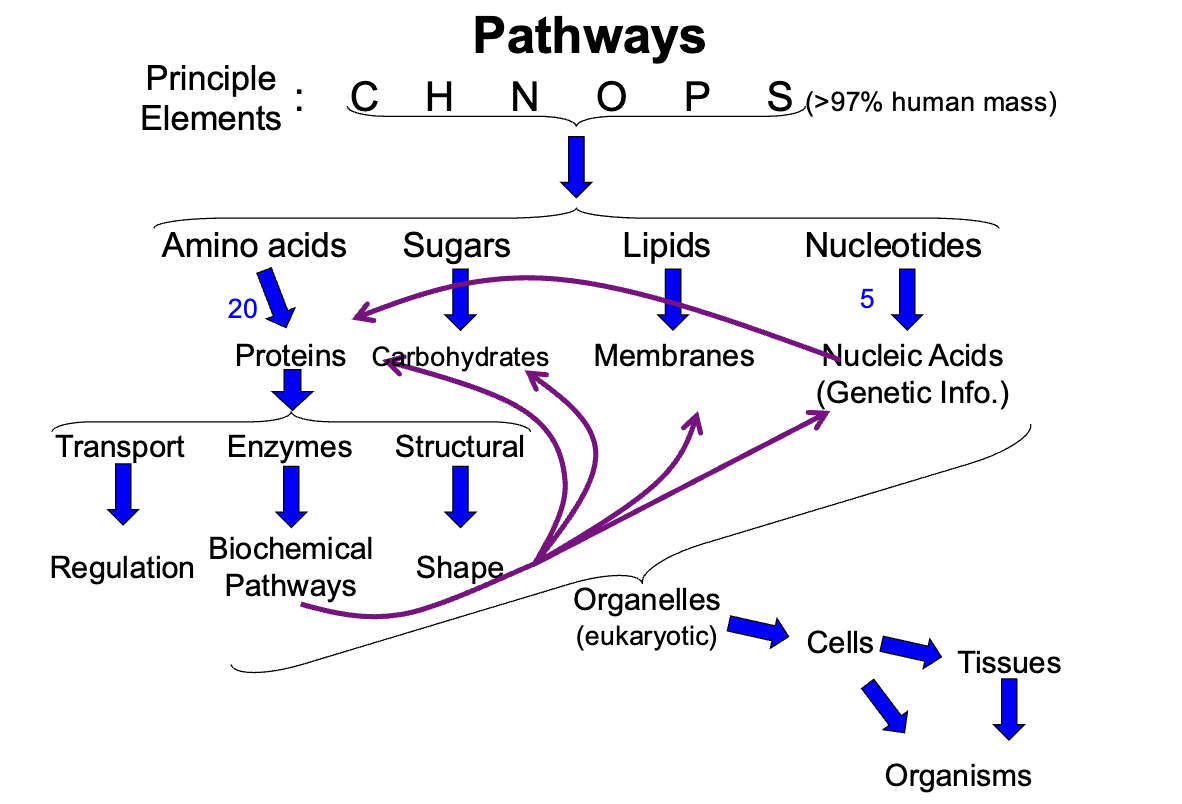
\includegraphics[width=0.8\textwidth]{pathways}
\end{figure}

\subsection*{Functional groups}

(R denotes a generic hydrocarbon chain)

Memorize!

\begin{figure}[H]
\centering
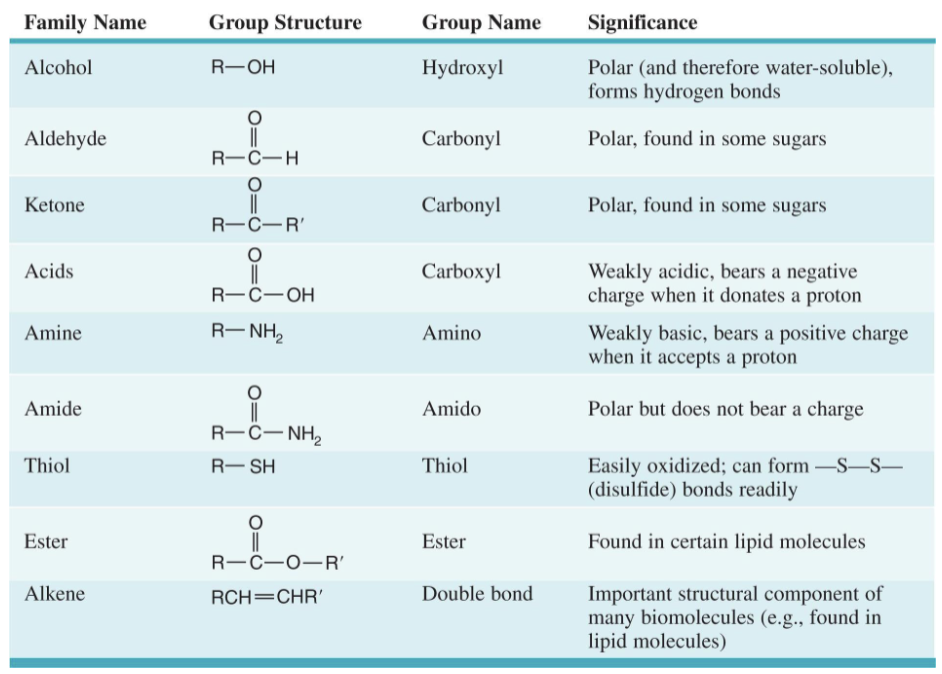
\includegraphics[width=0.8\textwidth]{functionalgroups}
\end{figure}

+ \textbf{phosphate} (\ce{PO4^3-})

\begin{itemize}
\item \textbf{Hydroxyl} + \textbf{carbonyl} $\to$ \textbf{carboxyl}
\item \textbf{Amine} + \textbf{carbonyl} $\to$ \textbf{amide}
\item \textbf{Aldehyde} has carboxyl at the \textbf{end}; \textbf{ketone} has it in the \textbf{middle}
\end{itemize}

\subsection*{Representations of molecules}

\begin{figure}[H]
\centering
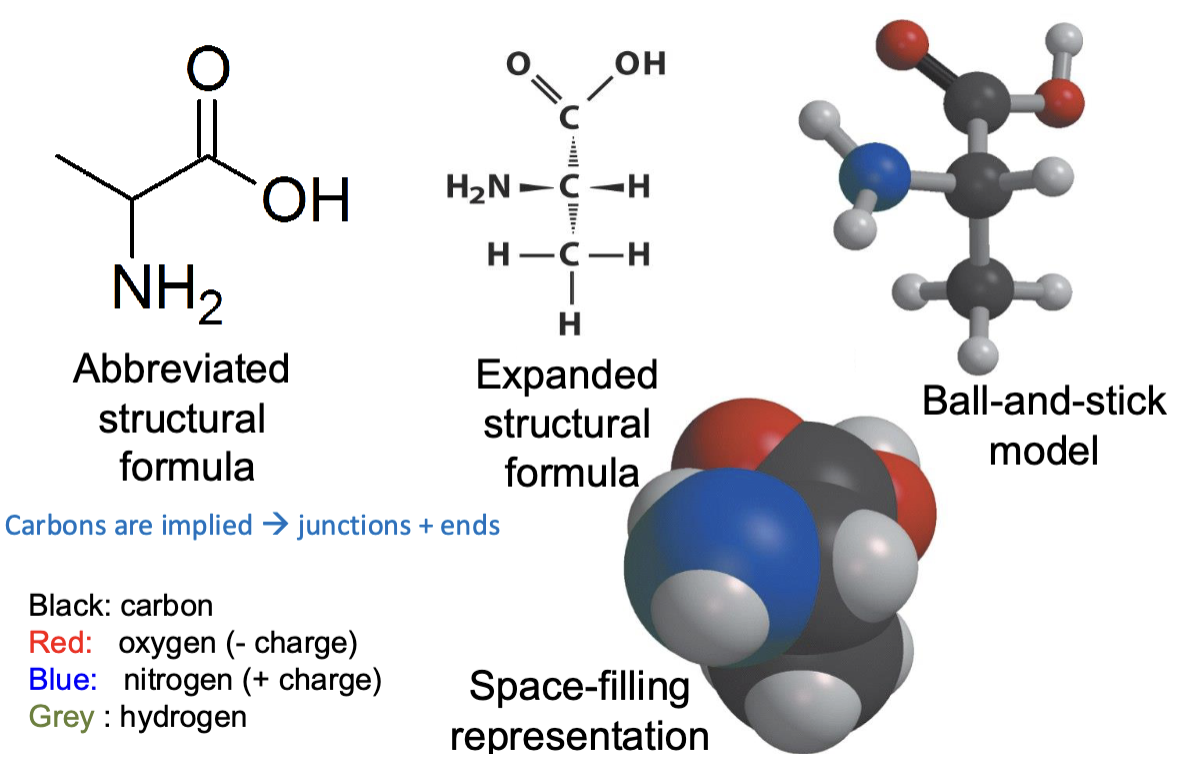
\includegraphics[width=0.8\textwidth]{models}
\end{figure}

\subsection*{The four major classes}

\subsubsection*{Amino acids}

\begin{itemize}
\item Hundreds of naturally occurring forms
\item Defined by the presence of amine and carboxylic acid groups
\item Classified based on the proximity of these groups
\item Three different classes: $\alpha$, $\beta$, and $\gamma$ based on which carbon is attached to the amine (closest to the central carbon is $\alpha$, next is $\gamma$, etc.)
\item $\alpha$ amino acid (most common): \textbf{amine} attached to \textbf{$\alpha$ carbon} (1 away from the central carbon), carboxyl and an \textbf{R group} (side chain, 20 different common types)
\item \textbf{Peptide} or \textbf{amide} bonds link amino acids together (form amide group with the carboxyl group + amine group)
\end{itemize}

\subsubsection*{Sugars (carbohydrates)}

\begin{itemize}
\item Molecules containing carbonyl and hydroxyl functional groups
\item Two classes: \textbf{ketose} and \textbf{aldose} sugars (carbonyl in the middle = ketose, at the end = aldose, same as functional groups)
\item Hydrated carbons
\item Very hydrophilic
\end{itemize}

\subsubsection*{Lipids}

\begin{itemize}
\item Soluble in hydrophobic solutions
\item Do not polymerize but form higher order structures
\item Fatty acids
\end{itemize}

\subsubsection*{Nucleotides}

\begin{itemize}
\item 3 basic components: phosphate group(s), ribose, nitrogenous base
\item Polymerize into: DNA (deoxyribose, adenosine, cytosine, guanine, thymine); RNA (ribose, adenosine, cytosine, guanine, uracil)
\item \textbf{Purines} (2 rings) and \textbf{pyrimidines} (1 ring)
\item Mnemonics: ``Pure As Gold'' (adenine and guanine are purines) and ``CUT the Py'' (cytosine, thymine, and uracil are pyrimidines)
\end{itemize}

\newpage

\section*{Water (\ce{H2O}): the biological solvent}

\subsection*{Physical properties of water}

\begin{itemize}
\item Solvent characteristics
\item Non-compressible
\item Chemical stability
\item Biochemical reactant
\item Hydration of molecules
\item Participates in biomolecular interactions
\item Ice floats
\item High boiling and freezing temperatures
\item High heat of vaporization
\item High specific heat capacity
\item High surface tension
\item Dissolves molecules with ionizable or polarizable functional groups but cannot dissolve nonpolar or hydrophobic molecules
\end{itemize}

\subsection*{Molecular properties of water}

\begin{itemize}
\item \textbf{Tetrahedral} electron geometry (104.5 degrees),  sp$^3$ hybridized, 0.99 Å from H to O
\item Electronegativity results in the formation of \textbf{polar bonds}
\item Forms \textbf{hydrogen bonds} (hydrogen is attracted to the lone pair electrons of an oxygen from another molecule)
\end{itemize}

\subsection*{Properties of hydrogen bonds}

\begin{itemize}
\item \textbf{Oxygen}, \textbf{nitrogen}, and \textbf{fluorine} can form hydrogen bonds (very electronegative)
\item Require a donor (has H attached) and acceptor (has free lone pair)
\item Hydrogen bonds in between casual interaction and covalent interaction in terms of proximity
\item Both covalent and electrostatic properties
\item Collinear orientation (present in a straight line)
\item Other orientations possible but not as strong
\item Electrostatic interaction
\item Atoms involved share electrons
\item In liquid water, 3.4 neighbors on average (4 in ice)
\item Hydrogen bonds can be disrupted by water
\end{itemize}

\subsection*{Weak interactions}

\begin{itemize}
\item Weak interactions are constantly being formed and broken between biomolecules (more transient)
\item Additive (can become strong)
\item Essential for rapid communication
\item Allows for flexibility
\item Three types of weak electrostatic interactions
\begin{itemize}
\item \textbf{Salt bridges} (ionic)
\item \textbf{Van der Waals interactions}
\item \textbf{Hydrogen bonds}
\end{itemize}
\end{itemize}

\subsection*{Relative strengths of interactions}
Strongest to weakest
\begin{itemize}
\item Int\textbf{ra}molecular forces
\begin{itemize}
\item Ionic bonds
\item Covalent bonds
\end{itemize}
\item Int\textbf{er}molecular forces (IMFs)
\begin{itemize}
\item Ionic interactions and salt bridges
\item Van der Waals forces:
\begin{itemize}
\item Hydrogen bonds
\item Dipole-dipole interactions
\item London dispersion forces (LDFs)
\end{itemize}
\end{itemize}
\end{itemize}

\subsubsection*{Salt bridges and ionic interactions}

\begin{itemize}
\item One positive interacting with one negative with full electrical charges (ionic bonds are NOT salt bridges)
\item Interaction strength calculated from Coulomb's law: $$ F = \frac{1}{4 \pi \varepsilon_0 } \frac{q_1q_2}{\varepsilon_r r^2}$$
\begin{itemize}
\item $F$ is interaction strength
\item $q_1$ and $q_2$ are signed charges
\item $r$ is the distance between centers
\item $\varepsilon_r$ is the dielectric constant
\item All others are constants
\end{itemize}
\item Water is good at breaking ionic bonds
\item \textbf{Hydration shells} prevent ionic bonds from reforming
\end{itemize}

\subsubsection*{Dipole interactions}

\begin{itemize}
\item Occur between molecules that have or can adopt a \textbf{dipole moment} ($\mu$)
\item Three types
\begin{itemize}
\item \textbf{Dipole-dipole interactions} (fixed dipoles)
\item \textbf{Dipole-induced dipole interactions} (fixed dipole and nonpolar)
\item \textbf{Induced dipole-induced dipole interactions (London Dispersion)} (nonpolar and nonpolar)
\end{itemize}
\end{itemize}

\subsubsection*{LDFS: a type of van der Waals interaction between non-polar molecules}

\begin{figure}[H]
\centering
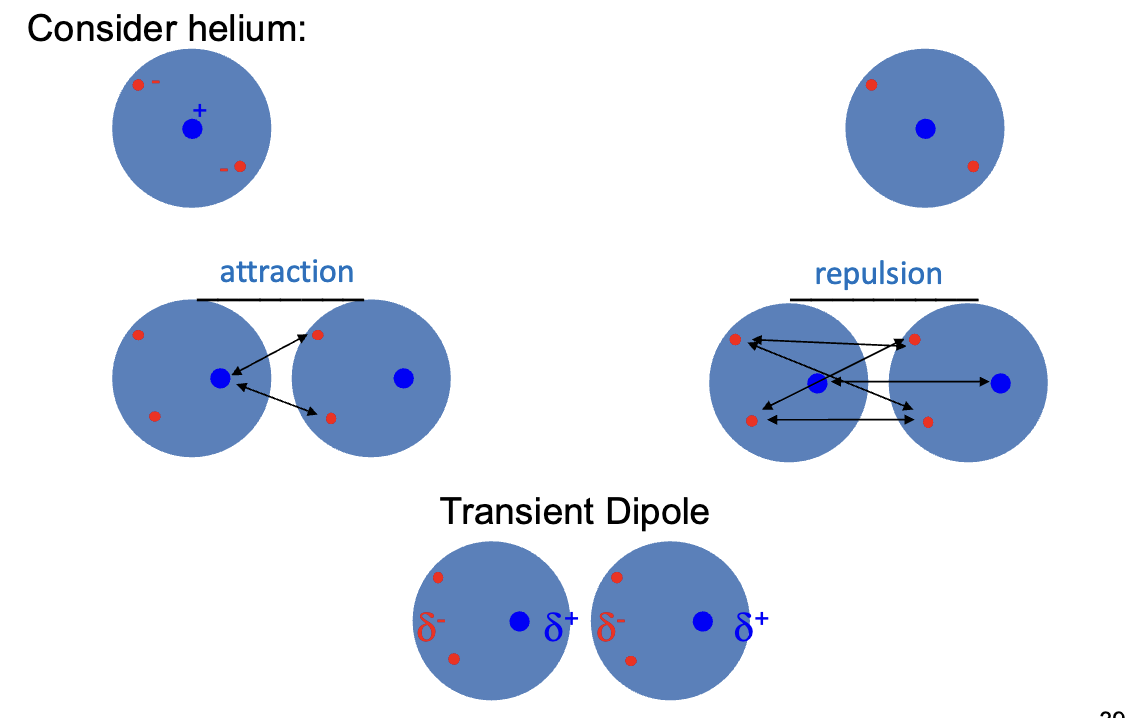
\includegraphics[width=0.8\textwidth]{ldfs}
\end{figure}

Electrons are constantly moving creating transient dipoles in nonpolar molecules

\subsection*{Lennard-Jones plot}

\begin{figure}[H]
\centering
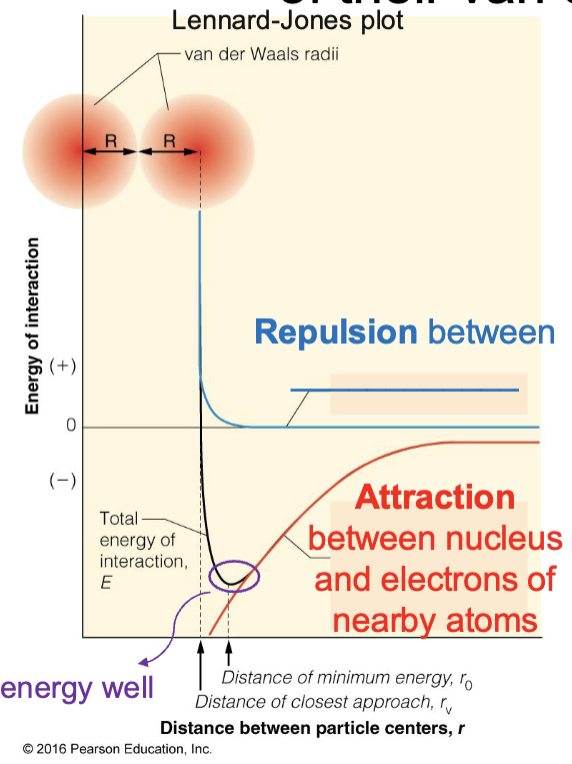
\includegraphics[width=0.6\textwidth]{lennardjones}
\end{figure}

Atoms come together until they reach the \textbf{van der Waals distance/radius} at which point they begin to repel each other

\subsection*{Hydrophobic molecules}

\begin{itemize}
\item Oil and water do not mix - oil is hydrophobic
\item Hydration shells will still form, but they are not stabilized
\item The separation of water and hydrophobic molecules is driven by the \textbf{hydrophobic effect}
\item Favorable because there is an increase in \textbf{entropy}
\item Second law of thermo: All spontaneous processes result in an overall increase of entropy in the universe ($\Delta S_\text{universe} >$ 0)
\item Nonpolar-nonpolar - shell of hydration, but less water that forms the shell. More water ends up in the system, increasing water entropy and increasing overall entropy (energetically favorable)
\item The overall entropy increases when only one cage is formed
\item Hydrophobic effect drives the folding of proteins
\item \textbf{Hydrophobic R-groups} are \textbf{forced into the core}; \textbf{hydrophilic R-groups form a shell} around the hydrophobic core. \textbf{Van der Waals forces organize amino acids} in the core
\item Molecules with hydrophilic and hydrophobic ``sides'' (example: phospholipids) forming micelles and bilayers
\end{itemize}

\subsection*{Hydrophobic effect vs. van der Waals}

\begin{figure}[H]
\centering
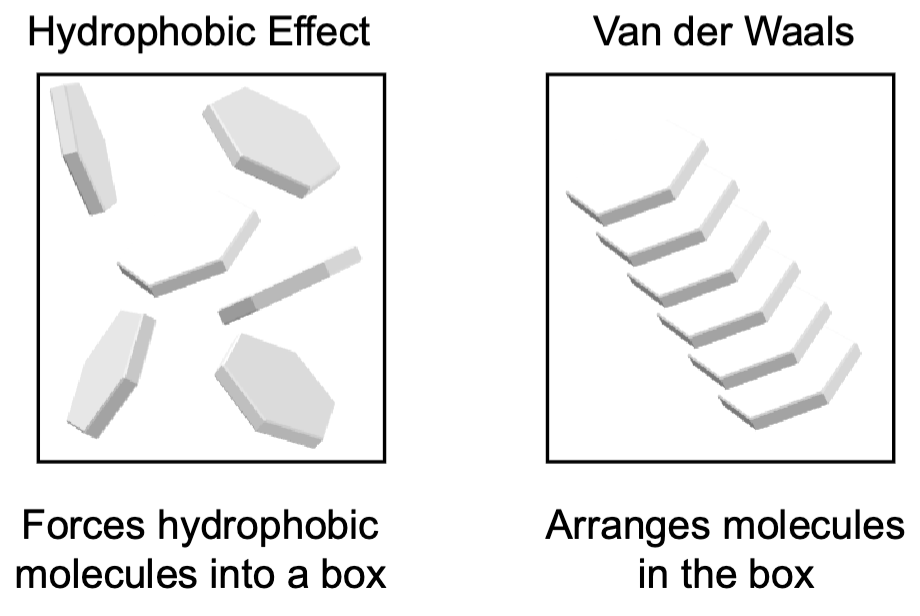
\includegraphics[width=0.7\textwidth]{hydrophobicvsvdw}
\end{figure}

\subsection*{pH}

\begin{itemize}
\item Hydrogen ions (H$^+$, ``protons'') can be gained or lost by some functional groups changing the properties of functional groups
\item pH is tightly regulated by the body at 7.4
\item A change greater than 0.5 pH units can lead to coma or death
\end{itemize}

A small amount of water ionizes: $$2 \ce{H2O}_{(l)} \rightleftharpoons  \ce{H3O+}_{(aq)} + \ce{OH-}_{(aq)}$$

For simplicity: $$\ce{H2O}_{(l)} \rightleftharpoons \ce{H+}_{(aq)} + \ce{OH-}_{(aq)}$$

\subsubsection*{Dissociation constant formula}

\begin{equation}
K_w = [\ce{H+}][\ce{OH-}]
\end{equation}

\subsubsection*{Calculation of pH and pOH}

\begin{equation} \label{pH}
\mathrm{pH} = -\log [\ce{H+}]
\end{equation}

\begin{equation}
\mathrm{pOH} = -\log [\ce{OH-}]
\end{equation}

\subsection*{Acids and bases}

\begin{itemize}
\item \textbf{Brønsted acids} are \ce{H+} donors
\item \textbf{Brønsted bases} are \ce{H+} acceptors
\item A \textbf{strong acid} or \textbf{strong base} is \textbf{completely ionized} in water ($A + B \to C + D$)
\item \textbf{Weak acids} are \textbf{incompletely ionized} in aqueous solutions ($A + B \rightleftharpoons C + D$)
\item Charges depend on the functional group
\item Acid becomes conjugate base; base becomes conjugate acid
\item Weak acid and its conjugate bases reach equilibrium in solution
\end{itemize}

\subsubsection*{Acid dissociation formula}

 \begin{equation}
K_a = \frac{[\ce{H+}][\text{conjugate base}]}{[\text{weak acid]}}
\end{equation}

Larger $K_a$ (dissociation constant) = stronger acid

\subsubsection*{ICE table (for weak acids only)}

\begin{table}[H]
\centering
\begin{tabular}{cccc}
Initial & 100 mmol & 0 & 0 \\
Change & -X & +X & +X \\
End & 100 mmol - X & +X & +X \\
\end{tabular}
\end{table}

\subsubsection*{Le Châtelier's Principle}

The degree to which a weak acid is dissociated depends on the pH of the system (if you decrease something, how does equilibrium shift?)

\begin{equation}
K_a = \frac{[\ce{H+}] [\ce{A-}]} {[\ce{HA}]}
\end{equation}

\subsection*{Titration}

A strong/weak acid or a strong/weak base is always titrated with a \textbf{strong acid/base} (neutralization reaction)

$$ \ce{HA} + \ce{OH} \rightleftharpoons \ce{A} + \ce{H2O} $$

\begin{itemize}
\item \textbf{Equivalence point} occurs when \textbf{all HA is neutralized}

\item \textbf{Half equivalence} happens halfway between the start and the equivalence point

\item Buffering is best on the flat part of the curve

\item pH (potential of hydrogen) = pKa (strength of weak acid)

\end{itemize}

Henderson-Hasselbach equation for weak acid/conjugate base or weak base/conjugate acid:

\begin{equation}
\text{pH} = \text{pKa} + \log \frac{[\ce{A+}]}{[\ce{HA}]}
\end{equation}

Maximum buffering capacity when [HA] = [A$^-$]

\subsubsection*{Buffers}
A buffer resists changes in pH. Buffers form weak acid/conjugate base or weak base/conjugate acid pairs.

Bicarbonate buffer is one of the more important buffers in blood.

$$\ce{CO2} + \ce{H2O} \rightleftharpoons \ce{H2CO3} \rightleftharpoons \ce{HCO3-} + \ce{H+}$$

\end{document}